% Use only LaTeX2e, calling the article.cls class and 12-point type.

\documentclass[12pt]{article}

% Users of the {thebibliography} environment or BibTeX should use the
% scicite.sty package, downloadable from *Science* at
% http://www.sciencemag.org/authors/preparing-manuscripts-using-latex
% This package should properly format in-text
% reference calls and reference-list numbers.

\usepackage{scicite}

\usepackage{times}

% Packages I manually added
\usepackage{graphicx}
\usepackage{placeins}
\usepackage{float}
\usepackage{amsmath}
\usepackage{hyperref}
\usepackage{pdflscape}



% The preamble here sets up a lot of new/revised commands and
% environments.  It's annoying, but please do *not* try to strip these
% out into a separate .sty file (which could lead to the loss of some
% information when we convert the file to other formats).  Instead, keep
% them in the preamble of your main LaTeX source file.


% The following parameters seem to provide a reasonable page setup.

\topmargin 0.0cm
\oddsidemargin 0.2cm
\textwidth 16cm
\textheight 21cm
\footskip 1.0cm


%The next command sets up an environment for the abstract to your paper.

\newenvironment{sciabstract}{%
\begin{quote} \bf}
{\end{quote}}



% Include your paper's title here

\title{Supplementary Materials for: ``Well-Designed Fishery Markets Enable Large-Scale Marine Conservation''}


% Place the author information here.  Please hand-code the contact
% information and notecalls; do *not* use \footnote commands.  Let the
% author contact information appear immediately below the author names
% as shown.  We would also prefer that you don't change the type-size
% settings shown here.

\author{Juan Carlos Villase\~{n}or-Derbez,$^{1\ast}$ John Lynham,$^{2}$ Christopher Costello$^{1}$\\
\\
\normalsize{$^{1}$Bren School of Environmental Science \& Management,}\\
\normalsize{University of California at Santa Barbara, Santa Barbara, CA}\\
\normalsize{$^{2}$Department of Economics, University of Hawaii at Manoa, Honolulu, HI}\\
\\
\normalsize{$^\ast$To whom correspondence should be addressed; E-mail: juancarlos@ucsb.edu.}
}

% Include the date command, but leave its argument blank.

\date{}



%%%%%%%%%%%%%%%%% END OF PREAMBLE %%%%%%%%%%%%%%%%



\begin{document}

% Double-space the manuscript.

\baselineskip24pt

% Make the title.

\maketitle


\newcommand{\beginsupplement}{\setcounter{table}{0}  \renewcommand{\thetable}{S\arabic{table}} \setcounter{figure}{0} \renewcommand{\thefigure}{S\arabic{figure}}}

\setcounter{table}{0}  \renewcommand{\thetable}{S\arabic{table}} \setcounter{figure}{0} \renewcommand{\thefigure}{S\arabic{figure}}

\section{Supplementary Materials}

\subsection{Model for marine conservation with effort markets}

We model a ten-patch discrete-time meta-population system, where Patch 1 is considering a spatial closure. Patches 1 - 9 operate under a vessel-day scheme, and Patch 10 represents the high seas and other areas not managed under a VDS. The stock of fish in each country is relatively stationary within a single fishing season, but  growth from escapement redistributes across all patches annually. The price of fish is $p$, and catchability is given by $q$. These parameters are held constant across patches.

Our purpose is to examine how the VDS affects a country's incentives for large-scale conservation. Suppose that Country 1 considers closing a portion $R$ (between 0 and 1) of its waters to all fishing; several consequences may arise. First, the area available to fish in Country 1 is now limited, which could reduce the amount of money fishing firms are willing to pay for a day of fishing in these waters. Second, to the extent that catch is reduced in Country 1, fish may become more abundant elsewhere; this could imply an increase in the lease price to fish in the other eight PNA countries' waters because the VDS price reflects the profit from fishing in a country, which depends crucially on the abundance of fish. For the same reason, the increase in abundance could attract new entrants on the high seas, who could quickly dissipate the benefits there. We focus on how design features of the market affect Country 1's incentives to create the marine reserve.

\subsubsection{Fishery dynamics}

In the absence of a reserve, the revenue for vessels in patch $i$ is given by $pqE_iX_i$, where $E_i$ and $X_i$ are effort (vessel-days) and stock size in patch $i$ at the beginning of a period. The cost of fishing in patch $i$ is given by $cE_i^\beta$, where $\beta = 1.3$ matches commonly-used cost functions.

Patch 1 considers a spatial closure by implementing a reserve as a fraction $R$ of the total patch ($R \in[0,1)$). Fish move within a patch based on $\theta$, where $\theta = 0$ implies no movement within the patch, and $\theta = 1$ implies that fish move so much that they can be caught from anywhere within the patch. In this patch, revenues are given by $pqE_1X_1(\theta + (1 - \theta)(1 - R))$. The parameterization of movement and reserve size imply that profit from fishing Patch 1 is given by:

$$
\Pi_1(E_1,X_1,R) = pqE_1X_1\Omega_1-cE_1^\beta
$$

\noindent with $\Omega_1 = (\theta + (1 - \theta)(1 - R))$ being a parameterization that combines reserve size as a proportion of patch ($R =  [0, 1)$) and within-patch fish movement ($\theta$). Under this parameterization, $\Omega_{i \neq 1} = 1$ since only Patch 1 implements a reserve.

Therefore, we can generalize the patch-level profit equation to:

$$
\Pi_i(E_i,X_i, R_i) = pqE_iX_i\Omega_i-cE_i^\beta
$$

\noindent The above equations imply that the marginal profit from the last unit of effort in a patch are given by:

\begin{equation}
\pi_i(E_i) = \frac{\partial \Pi_i}{\partial E_i} = pqX_i\Omega_i - \beta cE_i^{\beta-1}
\label{eqn:marginal_profit}
\end{equation}

In practice, the effort levels in each Patch are allocated by management (so $E_{1},\ E_{2},...,E_{9}$ are given) and the
effort level on the high seas ($E_{10}$) is a result of open access dynamics. Therefore, we assume that effort continues to enter Patch 10 until the profit from the last unit of effort is exactly zero, indicating that $E_{10}$ is the value for which $\pi_{10}(E_{10})  = 0$. Setting Equation \ref{eqn:marginal_profit} for $i = 10$ equal to zero and removing $\Omega_{10} = 1$ for simplicity, we can solve for $E_{10}$:

\begin{equation}
E_{10} = \left(\frac{pqX_{10}}{\beta c}\right)^{\frac{1}{(\beta - 1)}}
\label{eqn:effort_hs}
\end{equation}

Under VDS-operated patches, however, profits from the marginal unit of effort should equate to the price of fishing in the patch. Therefore vessel-day price for patches under VDS ($i = (1, 9)$) is  given by:

$$
\pi_i = pqX_i\Omega_i - \beta c E_i ^{\beta - 1}
$$

\noindent We can solve for $E_i$ and obtain:

\begin{equation}
	\begin{split}
		\pi_i + \beta c E_i ^{\beta - 1} &= pqX_i\Omega_i \\
		\beta c E_i ^{\beta - 1} &= pqX_i\Omega_i - \pi_i \\
		E_i ^{\beta - 1} &= \frac{pqX_i\Omega_i - \pi_i}{\beta c} \\
		E_i &= \left(\frac{pqX_i\Omega_i - \pi_i}{\beta c }\right) ^ {\frac{1}{\beta - 1}}
	\end{split}
\label{eqn:demands}
\end{equation}

Equation \ref{eqn:demands} tells us patch-level effort for a given patch-specific stock size ($X_i$) and vessel-day price ($\pi_i$). A vessel-day scheme establishes a cap on total effort allowed. This means that fishing effort from Patches 1 - 9 must add up to this limit. Therefore, total allowable effort in the fishery is given by:

\begin{equation}
\bar{E} = \sum_{i = 1}^9\left(\frac{pqX_i\Omega_i - \pi}{\beta c }\right) ^ {\frac{1}{\beta - 1}}
\label{eqn:Ebar}
\end{equation}

\noindent In the above Equation, vessel-day price is the same across all patches when trading is allowed; the subindex is dropped for this parameter.

\subsubsection{Stock dynamics}

Patch-level harvest is then determined by effort and stock size:

\begin{equation}
H_i = qE_iX_i\Omega_i
\label{eqn:harvest}
\end{equation}


\noindent Therefore, escapement in patch $i$ in time period $t$ is the difference between initial stock size and harvest given by $e_{i,t} = X_{i,t} - H_{i,t}$ and total escapement is $e_t=\sum_{i=1}^{10}e_{i,t}$. The entire stock then grows logistically according to:

\begin{equation}
X_{t+1} = e_t \times  e^{r \left(1 - \frac{e_t}{K} \right)}
\label{eqn:grow}
\end{equation}

\noindent where $r$ and $K$ are species-specific intrinsic growth rate and carrying capacity. After the stock grows, a constant and patch-specific fraction $f_i$ of the total stock redistributes to patch $i$, so:

\begin{equation}
X_{i,t+1} = f_iX_{t+1}
\label{eqn:disperse}
\end{equation}

\subsubsection{Vessel-day revenues}

The vessel-day price that a country charges is given by $\pi_i$ from Eqn \ref{eqn:marginal_profit}. Therefore, patch-level license revenues are given by:

\begin{equation}
\omega_i = \pi_iE_i
\label{eqn:license_revenue}
\end{equation}

\noindent Equation \ref{eqn:harvest} shows that low values of $\theta$ and $R > 0$ would decrease harvest and increase escapement in Patch 1, for a given level of effort and stock size. This would lead to an increase in total stock size (Equation \ref{eqn:grow}) and a benefit to all the other patches. But this would also cause the stock in the high seas ($X_{10}$) to increase, leading to increased effort being allocated to the high seas (Equation \ref{eqn:effort_hs}) and a loss of these potential rents. Thus, the spillover benefits of increasing $R$ are never completely captured.

\subsubsection{Simulations and parameterization}

We calibrate our model to loosely match the fishery dynamics observed for the VDS operated by the PNA. The table below contains the values used to parameterize the model.

\begin{table}[H]
\centering
\resizebox{\linewidth}{!}{
\begin{tabular}{l|r|l}
\hline
Parameter & Value & Source\\
\hline
MSY & 1.875600e+06 & 50th percentile from MSY in Table 8 of WCPFC Stock Assessment\\
\hline
$B_{msy}$ & 1.628000e+06 & 50th percentile from MSY in Table 8 of WCPFC Stock Assessment\\
\hline
K & 6.876526e+06 & 50th percentile from MSY in Table 8 of WCPFC Stock Assessment\\
\hline
$B_c/B_{msy}$ & 5.100000e-01 & 50th percentile from MSY in Table 8 of WCPFC Stock Assessment\\
\hline
$C_{now}$ & 1.679444e+06 & Catches from WCPFC Stock Assessment\\
\hline
$B_{now}$ & 3.507028e+06 & Current Biomass (2012 - 2015 average)\\
\hline
$r$ & 5.700000e-01 & From Fishbase: Prior r = 0.57, 95 CL = 0.41 - 0.78\\
\hline
$\beta$ & 1.300000e+00 & Standard\\
\hline
p & 1.100000e+03 & Mean between Thailand and Japan values (Value of WCPFC-CA Tuna Fisheries 2017 Report)\\
\hline
q & 3.420000e-05 & Estimated so that efforts match catches given biomass and vessel-day prices\\
\hline
c & 1.800000e+02 & -\\
\hline
f & 1.000000e-01 & Biomass is equally distributed between patches ($f_i = 0.1$)\\
\hline
\end{tabular}}
\end{table}

\noindent We run simulations under two market designs and test the model across a range of reserve sizes and within-patch movement parameters.The first scenario does not allow trading. In this case, total allowable effort ($\bar{E}$) and biomass $B_{now}$ are known and equally distributed among patches 1-9. For patch 10, we solve for Eq \ref{eqn:effort_hs} until biomass converges to match $B_{now}$. We then proceed to ``close'' a portion of Patch 1, and calculate the vessel-day price in Patch 1 given that only $X_i\Omega_i$ biomass is available for harvest. We compare vessel-day revenues of each scenario to a case with no reserve ($R = 0$). This produces a measure of the cost of implementing a spatial closure of size $R$ in Patch 1.

The second scenario allows trading. We start again by solving for the high seas to obtain total effort. Since a closure is not in effect and VDS-managed effort is equally distributed across the 9 patches, this equilibrium is the same as the first step above. We then implement a spatial closure in Patch 1. This essentially lowers the price fishers would be willing to pay to fish in a patch with only biomass $X_i\Omega_i$, lowering demand for vessel-days in Patch 1. Patches 2 - 9 have a higher demand for vessel days, and therefore a portion of vessel-days from Patch 1 are sold to Patches 2 - 9. This increases effort in these patches, which reduces escapement and therefore biomass. This reduction in biomass in turn will modify the marginal profit and willingness to pay to fish in each country. We therefore iterate this process until biomass stabilizes, finding the system's equilibrium. Like before, we calculate vessel-day revenues to each patch and compare them to a case with no reserve in Patch 1.

Annual vessel-days are often allocated based on a combination of historical within-patch effort and biomass. In the PNA, for example, 60\% of the allocation is calculated based on EEZ effort over the last seven years and 40\% is calculated based on the 10-year average of each country’s share of estimated skipjack and yellowfin biomass within its EEZ.\footnote{This is explained in more detail in Article 12.5 of the 2012 Amendment to the Palau Agreement and in \cite{Hagrannsoknir2014}.} Trading vessel-days to other countries would imply that historical within-patch effort declines through time. The allocated days to a patch with a full spatial closure would eventually be reduced to just the 40\% based on biomass.

In the trading scenario above, effort from Patch 1 (with the reserve) is traded to other patches. This means that its allocation will decrease as purse seine effort in its EEZ is reduced. After solving for the new equilibrium for each combination of $R$ and $\theta$, we project the fishery forward 50 years in time. At the end of every time period (a year), vessel-days are re-allocated to each patch based on the following rule:

$$
E_{i,t+1}^* = \alpha
\left(\frac{\sum_{\tau = 0}^{\hat{\tau}}E_{i,t-\tau}}{\sum_{\tau = 0}^{\hat{\tau}}\bar{E}_{{t-\tau}}}
	\right)
	+
(1 - \alpha)
\left(\frac{\sum_{\tau = 0}^{\hat{\tau}}X_{i,t-\tau}}{\sum_{\tau = 0}^{\hat{\tau}}\bar{X}_{t-\tau}} \right)
$$

\noindent where $\alpha$ is a weight on historical effort ($E_i$) and $1-\alpha$ is the weight on historical biomass ($B_i$). We use $\hat{\tau}= 6$ to obtain a moving mean of 7 years for these measures. The difference between allocated days ($E_i^*$) and used days (determined by Equation \ref{eqn:demands}) for Patch 1 are the sales. We then calculate vessel-day revenues to each country over the 50-year time horizon and compare to a case where there is no reserve and allocations are based solely on biomass ($\alpha = 0$).

\subsection{Data}

Automatic Identification Systems (AIS) are on-board devices that provide at-sea safety and prevent ship collisions by broadcasting vessel position, course, and activity to surrounding vessels. These broadcast messages can be received by satellites and land-based antennas. GFW then uses machine learning algorithms (convolutional neural networks) on the broadcast messages to infer type and location of fishing events \cite{kroodsma_2018}.

The amount of data gathered by GFW is dependent on the number of antennas and satellites that can receive signals. The total satellite count increased from 3 to 6 on June 1\textsuperscript{st} 2014, and then from 6 to 10 on January 1\textsuperscript{st} 2016. This causes an increase in the number of \emph{received} AIS messages (\emph{i.e.} points), and therefore an apparent increase in the number of vessels and vessel activity. The addition of new satellites affects all vessels in the same way.

Our displaced group contains all purse seiners (n = 64) that fished within PIPA at least once before the announcement, and that continued to fish elsewhere after the January 2015 implementation. Vessels in the non-displaced group meet the following two conditions: i) never fished within PIPA waters from 2012-2015, and ii) vessels have fished in surrounding areas (\emph{i.e.} PNA-countries' EEZ) before and after PIPA closure (n = 28). Together, these vessels represent more than 20 million geo-referenced positions for which we know activity (fishing or not fishing). We perform three sample restrictions as a robustness check. The first restriction excludes all Chinese vessels, the second excludes all PNA vessels, and the third excludes US and Taiwanese vessels.

Shapefiles of Exclusive Economic Zones were obtained through Marine Ecoregions of The World, we use World EEZ v10 (2018-02-21) available for download at: http://www.marineregions.org Shapefiles for Marine Protected Areas (PIPA and PNMS) come from the World Database of Protected Areas, and were downloaded in March 2019 from: https://www.protectedplanet.net.

\subsection{Empirical Analysis}

ENSO events are known to drive the location of fish and the behavior of fishing vessels, especially in PNA waters \cite{lehodey_1997,kroodsma_2018,aqorau_2018}. We do our best to control for these environmental changes by incorporating the NINO4 anomaly index in our analyses, and by tracking the non-displaced vessels as a ``control'' group that is equally affected by the environmental variation. For example, we observe that both displaced and non-displaced vessels shifted their effort post-PIPA to the Western margin of the PNA region, namely Kiribati's Gilbert Islands and Tuvalu. However, displaced vessels redistribute a greater proportion of fishing effort to these areas, as well as the High Seas (Fig \ref{fig:fishing_raster_diff}). Our analysis shows that sea surface temperature variation does have an effect on our crowding and behavioral outcomes, but that by itself it does not explain the observed patterns. While environmental variation certainly influences fishing behavior, policy and management interventions such as moratoriums and spatial closures can have even larger effects \cite{kroodsma_2018}.  Our analyses incorporate the monthly NINO4 anomaly index (Fig. \ref{fig:nino_plot}) to control for the responses that fish and vessels might have to environmental variation \cite{lehodey_1997,kroodsma_2018,aqorau_2018}.

\subsubsection{Behavioral changes}

We attempt to identify the response of vessels to the PIPA closure. We use daily fishing and non-fishing hours, daily proportion of fishing vs. non-fishing hours, daily distance traveled (km), distance from shore (km) and distance from home port (km) for fishing events, and proportion of total fishing hours allocated to Kiribati waters and PNA waters as our main outcomes of interest (Figure \ref{fig:all_panels}). We compare these outcomes before and after the implementation of PIPA using a Difference-in-Differences approach.

Our main specification is the following:

$$
log(y_{i,t}) = \alpha + \beta_1 P_t + \beta_2 D_i + \beta_3 P_t \times D_i + \phi_t + \gamma_i + \epsilon_{i,t}
\label{eqn:did}
$$

\noindent where $log(y_{i,t})$ is the hyperbolic-sine transformation\footnote{$ln\left(y + \sqrt{1 + y^2}\right)\rightarrow ln(2y)$. The transformation was not applied to the proportion of fishing to non-fishing hours.} of the outcome of interest for vessel $i$ in period $t$. A dummy variable $P_t$ takes the value of 0 for all dates prior to PIPA implementation and a value of 1 for all dates following PIPA implementation. $D_i$ is a dummy variable indicating whether a vessel belongs to the displaced ($D_i = 1$) or non-displaced ($D_i = 0$) group. $\alpha$ is the standard intercept term, $\beta_1$ captures the temporal trend, $\beta_2$ captures the initial difference between displaced and non-displaced groups, and $\beta_3$ is our parameter of interest: the difference-in-differences estimate capturing the treatment effect. Finally, $\phi_t$ and $\gamma_i$ represent month and flag dummies that account for seasonality or country-level management interventions. All regression coefficients were estimated via ordinary least squares, and heteroskedasticity-robust standard errors were calculated (Table \ref{tab:main_DID}).

We find no evidence of displaced vessels fishing more after the implementation and, in fact, observe a 27.5\% decrease relative to non-displaced vessels ($p < 0.01$; Fig. \ref{fig:all_panels}; Table \ref{tab:main_DID}). Likewise, we observe a 3.4\% decrease in fishing hours relative to total at-sea hours ($p < 0.01$). Displaced vessels traveled 23.3\% less distance, and fishing events occurred 32.9\% and 16.9\% closer to shore and to port, respectively. These changes in distance from shore and port are likely explained by redistribution, as we observe that displaced vessels fished less in Kiribati and PNA waters, compared to the trend observed for non-displaced vessels ($p < 0.01$). We do not observe changes in non-fishing at-sea hours (\emph{i.e.} a proxy for search time) and fishing hours on the High Seas. We repeat this analysis for sample restrictions where we exclude all Chinese vessels (Table \ref{tab:DID_without_CHN}), all PNA-owned vessels (Table \ref{tab:DID_without_PNA}) and all Taiwanese and USA vessels (Table \ref{tab:DID_without_USA_TWN}) and find qualitatively the same responses.

\subsubsection{Crowding effect}

\begin{equation}
y_t = \alpha + \beta_1 M_t + \beta_2 M_t^2 + \beta_3 M_t^3 + \beta_4 M_t ^4 + \sigma_s + \mu N_t + \epsilon_t
\label{eqn:sp_corr}
\end{equation}

We test for a crowding effect using the specification in Equation \ref{eqn:sp_corr}. We have two different outcome variables:
1) the number of cells that had fishing activity from displaced and non-displaced vessels per month and 2) the correlation of presence/absence of fishing events between both groups over one month.We allow for the possibility of three inflection points: 1) initial crowding due to MPA implementation, 2) When the crowding has reached its peak and starts to decrease, and 3) when this decrease potentially levels off. For this reason, we fit a 4th degree polynomial to our monthly indices. We do so by centering our time series of crowding indices on the day of implementation. Our explanatory variable is therefore the number of months ($M$) before or after the implementation. For example, since PIPA was implemented on January 1\textsuperscript{st} of 2015, December of 2014 has a value of -1 and Feb of 2015 would receive a value of 1. Note that we restrict the sample to our displaced and non-displaced vessels (vessels that show up in the dataset before PIPA implementation) to try to minimize bias from more and more vessels using AIS over time. We also include controls ($\sigma_s$) that captures the effect of additional satellites receiving AIS signals, which occurred on April 1st, 2014 and December 31st, 2015. The $\mu$ coefficient captures the effect of the NINO4 anomaly.

We inspect the crowding effects that may arise by applying more (or the same) fishing effort over less fishing area by inspecting the spatial overlap between displaced and non-displaced vessels over a gridded surface (Fig \ref{fig:fishing_raster_diff}). These groups interacted more with each other after the implementation of PIPA (Table \ref{tab:sp_corr}, Fig. \ref{fig:sp_corr}). The number of cells with presence from both fleets and the spatial correlation between groups increases by a factor of four and three, respectively. Environmental variation may certainly drive this, but the NINO4 anomaly alone explained just 3\% and 7\% of the variation in our crowding measures, compared to the 70\% variation explained when accounting for PIPA implementation (Table \ref{tab:sp_corr}). We observe similar patterns when replicating the crowding exercise for Kiribati's EEZ only (Table \ref{tab:KIR_sp_corr}, Fig \ref{fig:KIR_sp_corr}).

\subsubsection{Effort redistribution}

We can compare the footprint of displaced and non-displaced vessels before and after the implementation of PIPA to better understand the effort redistribution. Non-displaced vessels serve as a control group that was not subject to a spatial closure but might have redistributed in response to changing environmental conditions, such as ENSO. The spatial redistribution patterns of displaced vessels relative to non-displaced vessels suggest that some relocated to other waters in Kiribati (\emph{i.e.} Gilbert islands and Line islands), but also the Marshall Islands, Tuvalu, Nauru, and the high seas (Fig \ref{fig:fishing_raster_diff}).


\subsubsection{Revenues and catches}

We obtained information on revenues from the Pacific Islands Forum Fisheries Agency \emph{Tuna Development Indicators 2016} report.  Specifically, we use data compiled by the Pacific Islands Forum Fisheries Agency\footnote{https://www.ffa.int/node/2050} (FFA) where annual revenues from license fees (for VDS and other access programs) are reported for each country (2008 - 2016; Fig. \ref{fig:empirical}A). For countries in the PNA, these revenues show a combination of vessel-day license fees as well as joint-venture operations.

Total purse seine catch for each country's EEZ for the 1997 - 2016 period were also obtained from the FFA (Fig. \ref{fig:catches}). Catches in Kiribati waters decreased from 24,051 to 12,894 tonnes between 2015 and 2016 (46.3\% decrease). Similar decreases were observed for The Federated States of Micronesia (60.9\%), Papua New Guinea (43.4\%) and the Solomon Islands (58.5\%). In contrast, Tokelau (due south of PIPA) showed a 22.3\% increase in purse seine catch over the same period.

\subsubsection{Data and code availability}

All analyses were performed in R version 3.5.3 \cite{rcore_2018}. Raw data and code used in this work are available on \href{https://github.com/jcvdav/MPA_displacement}{github}.

\clearpage

\FloatBarrier

\section{Supplementary tables and figures}

\begin{figure}[htbp]
\centering
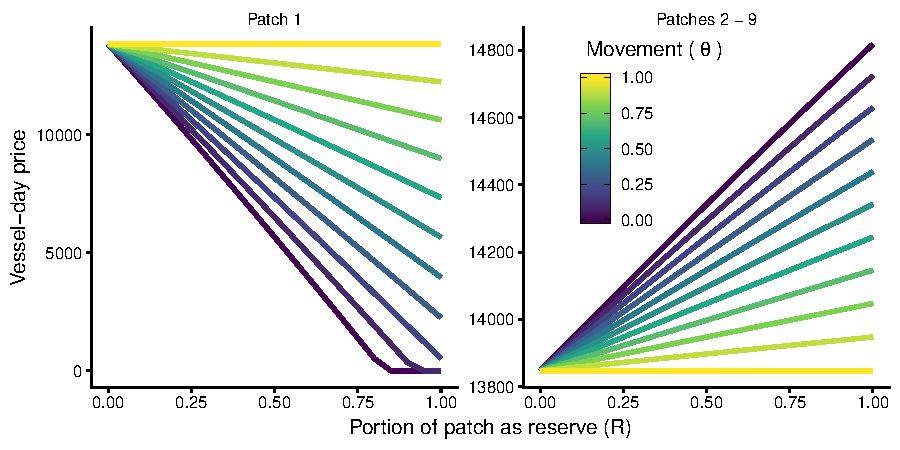
\includegraphics{img/vessel_day_price_no_trading_plot.pdf}
\caption{\label{fig:vessel_day_price_no_trading_plot}Vessel-day prices (vertical axis) for a combination of reserve sizes ($R$ in the horizontal-axis) and different within-patch movement ($\theta$) for the patch with spatial closure and other patches (left - right, respectively) when there is no trading.}
\end{figure}

\begin{figure}[htbp]
\centering
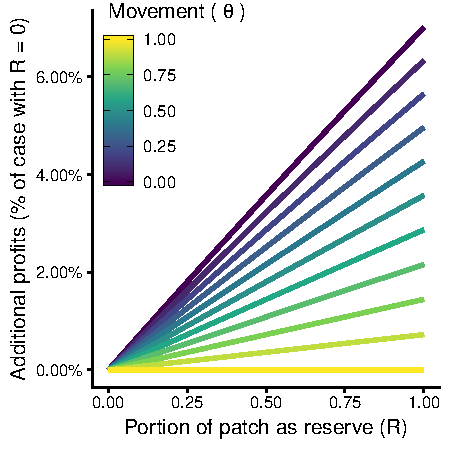
\includegraphics{img/profits_PNA_notKIR_no_trading_plot.pdf}
\caption{\label{fig:profits_PNA_notKIR_no_trading_plot}Relative change in revenue for patches 2 - 9 (vertical axis) for a combination of reserve sizes ($R$ in the horizontal-axis) and different within-patch movement ($\theta$) when there is no trading.}
\end{figure}

\begin{figure}
\centering
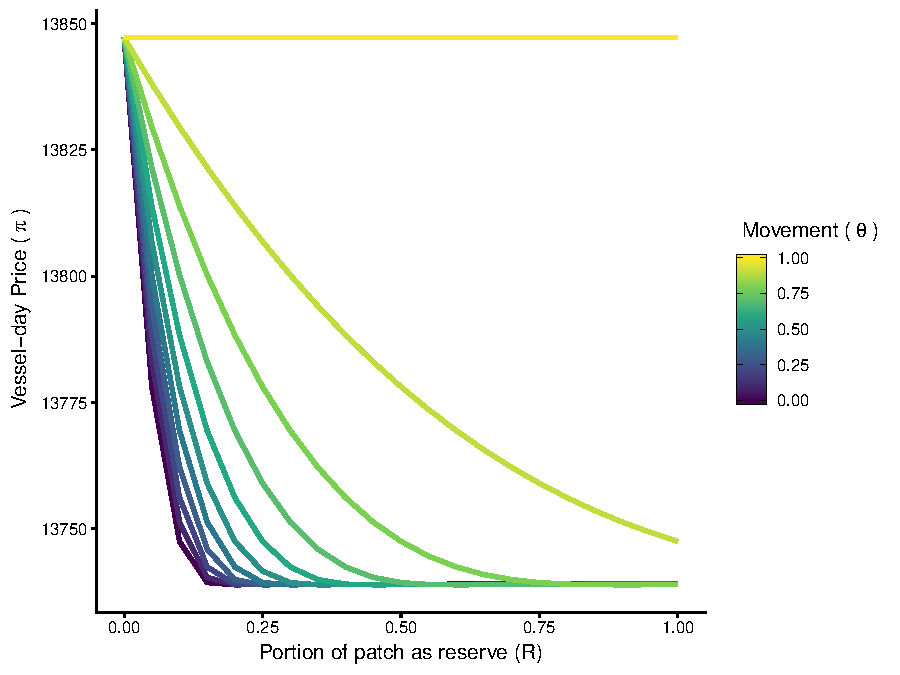
\includegraphics{img/vessel_day_price_with_trading_plot.pdf}
\caption{\label{fig:vessel_day_price_with_trading_plot}Vessel-day prices (vertical axis) for a combination of reserve sizes ($R$ in the horizontal-axis) and different within-patch movement ($\theta$) for the patch with spatial closure and other patches (left - right, respectively) when there is no trading.}
\end{figure}

\begin{figure}
	\centering
	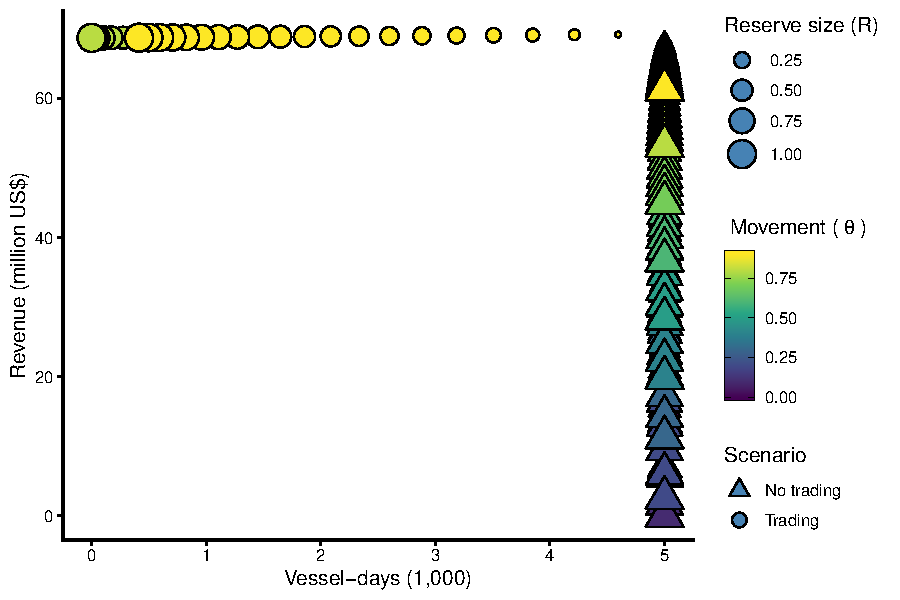
\includegraphics{img/effort_and_revenues.pdf}
	\caption{\label{fig:effort_and_revenues}Effort and revenue in Patch 1 for a combination of reserve sizes ($R$), different within-patch movement ($\theta$), and with and without trading. With trading, the relative drop in effort is always larger than the relative drop in revenue as $R$ increases. The exact opposite relationship holds without trading: effort remains fixed as revenue declines with increasing $R$.}
\end{figure}

\begin{figure}
\centering
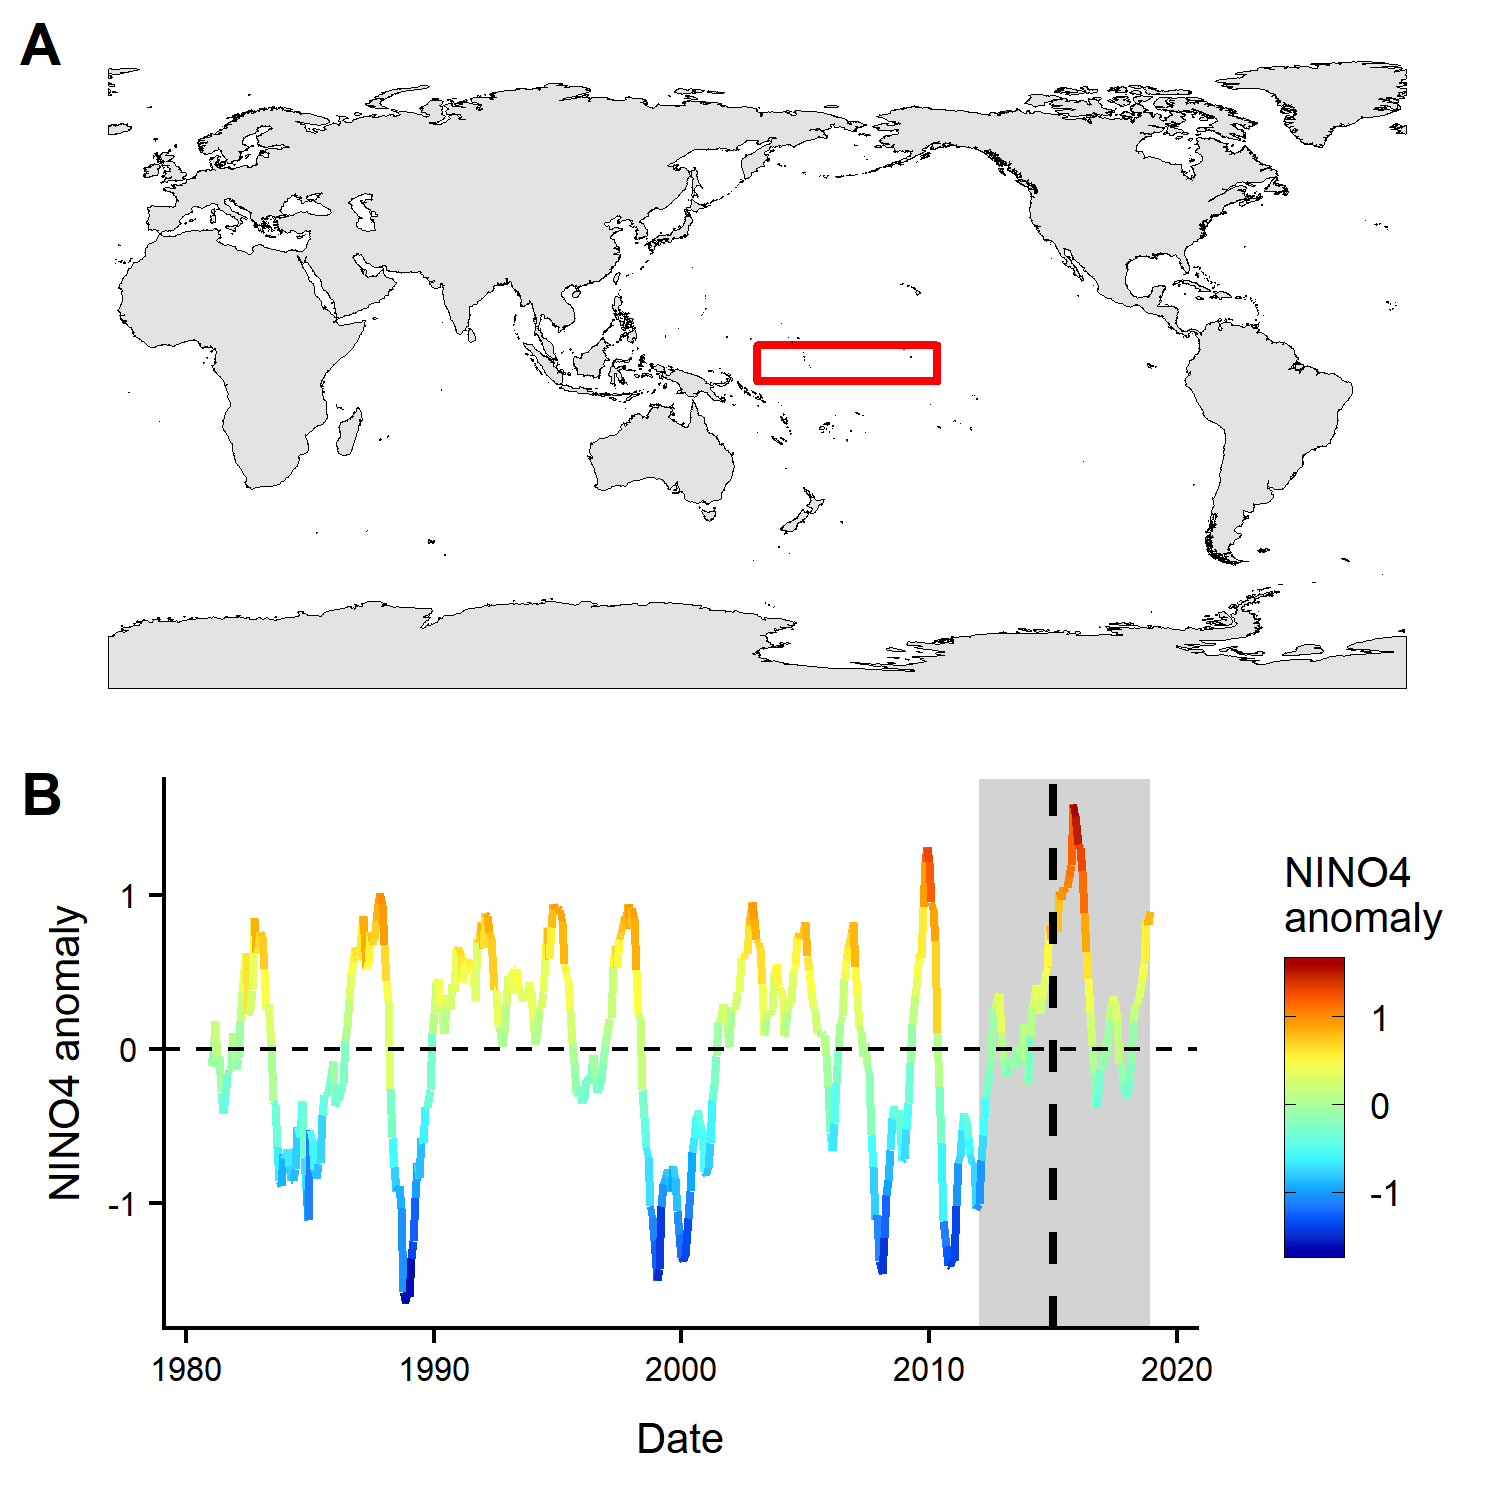
\includegraphics{img/nino_plot.png}
\caption{\label{fig:nino_plot}NINO4 anomaly index. A) Map of the NINO4 region (5S-5N and 160E-150W). B) Time series of NINO4 anomaly from January, 1980 to December, 2018.}
\end{figure}

\begin{figure}
\centering
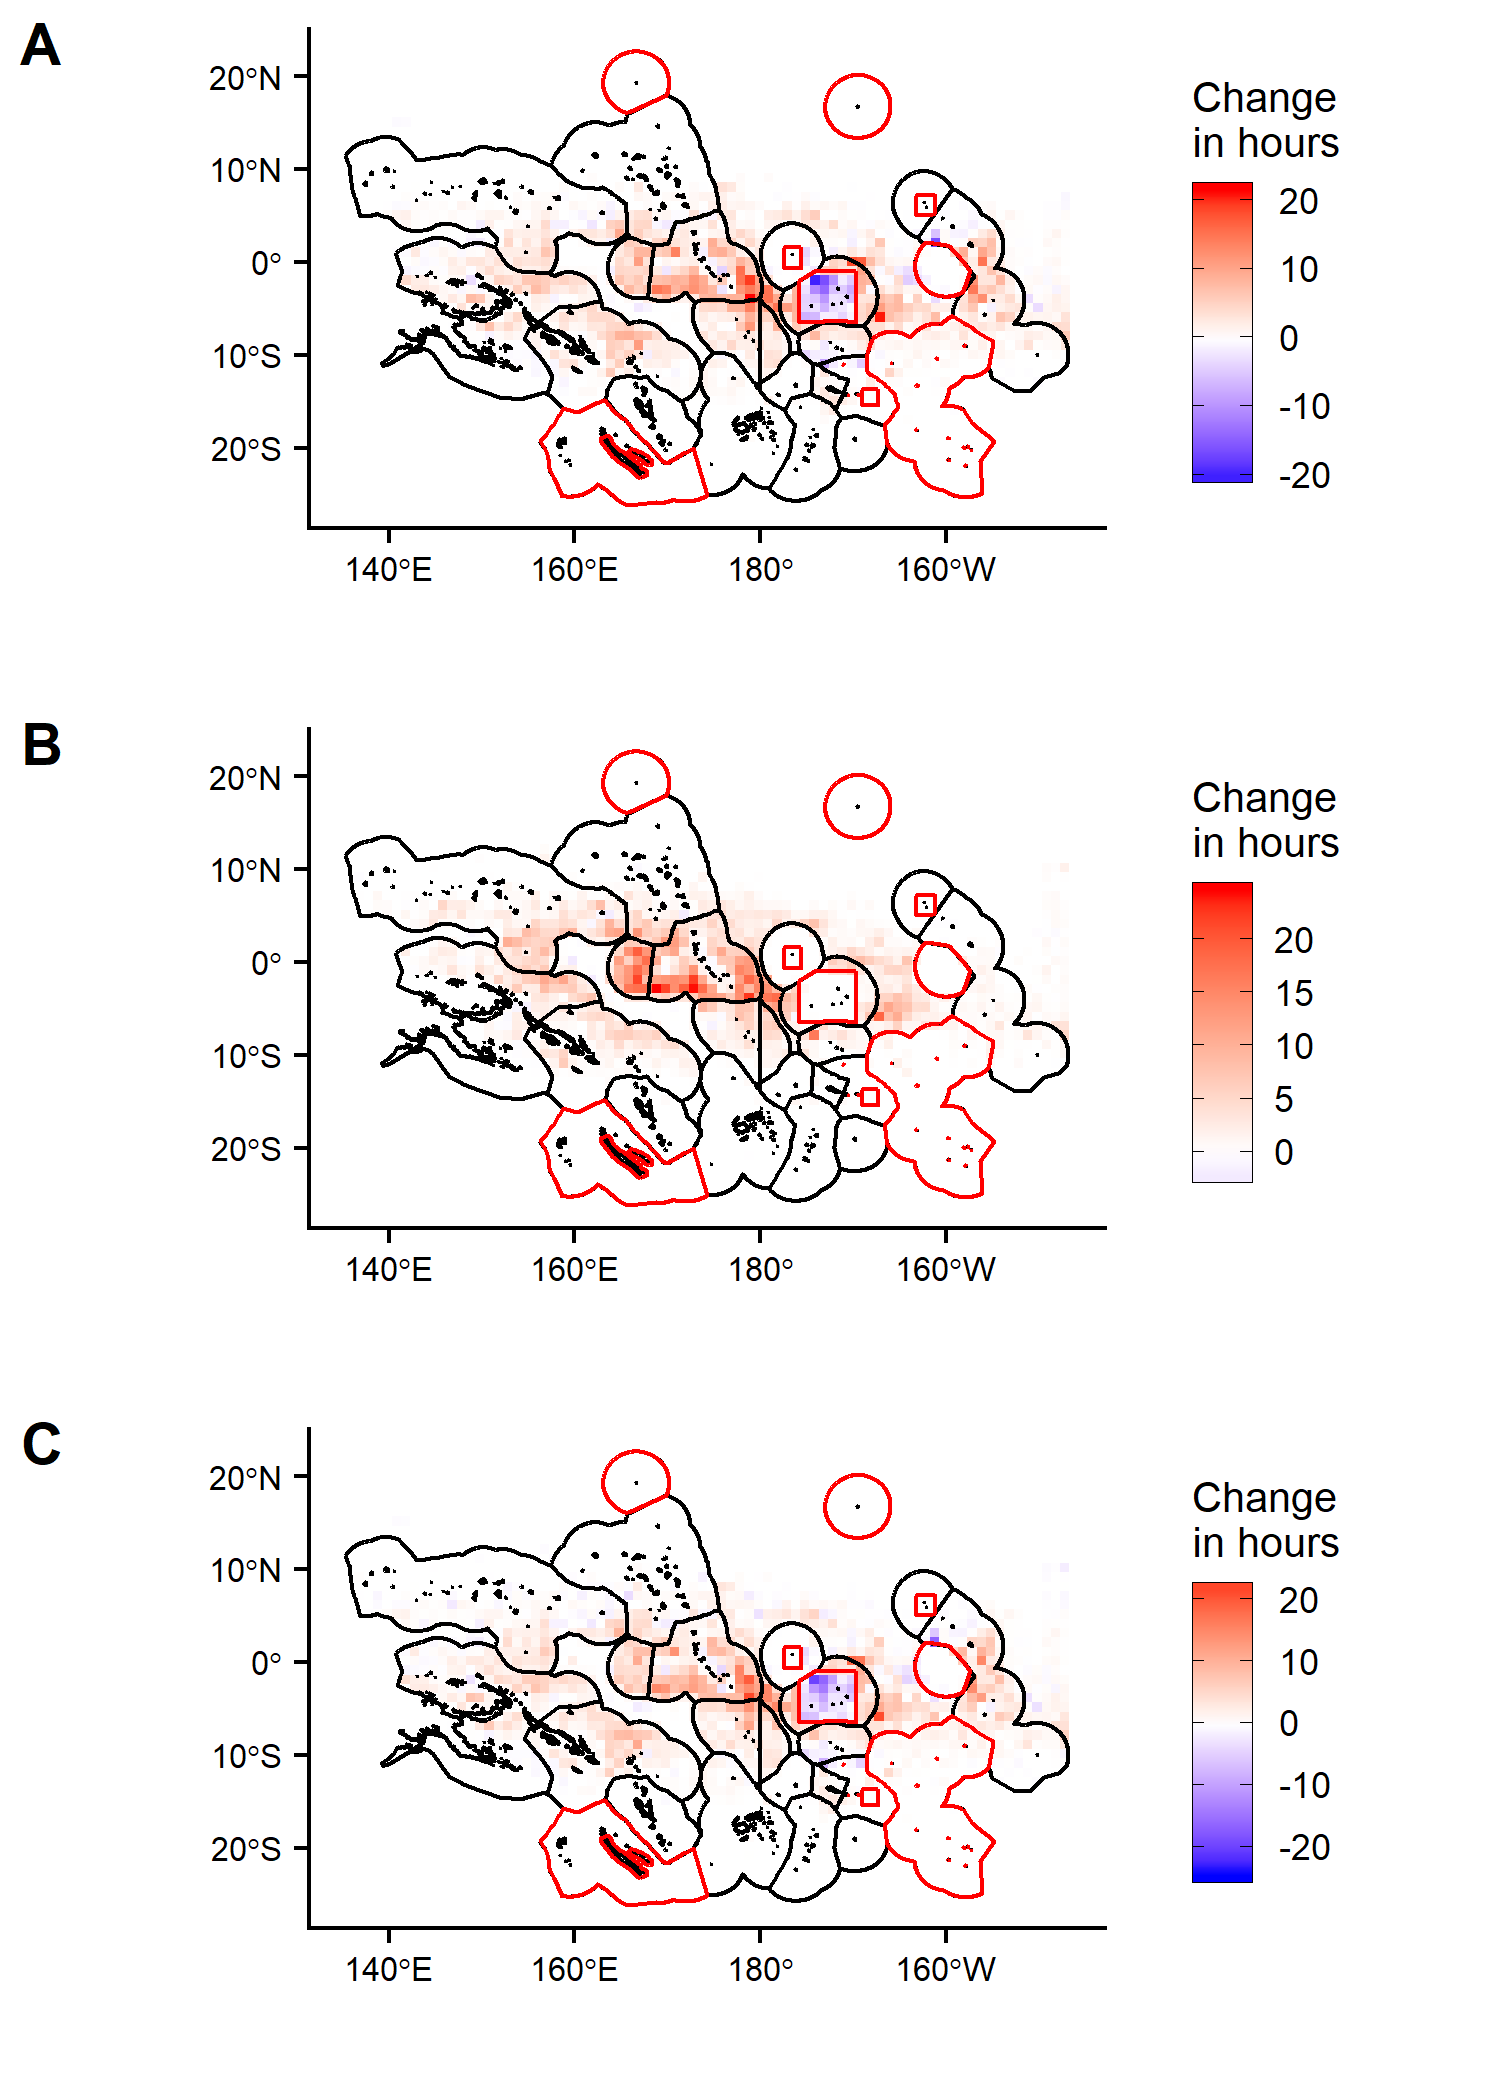
\includegraphics{img/fishing_raster_diff.png}
\caption{\label{fig:fishing_raster_diff}Change in spatial footprint of analyzed vessels. Black lines show Exclusive Economic Zone (EEZ), red lines show Marine Protected Areas. Panels A and B show the change through time (after - before) for displaced (A) and non-displaced vessels (B). Panel C shows the difference between A and B (displaced - non-displaced), highlighting areas where displaced vessels redistributed to, relative to non-displaced vessels. Note that displaced vessels allocate more hours to the Gilbert Islands and Line islands EEZs, but also Tuvalu and the high seas surrounding PIPA and Kiribati's EEZ.}
\end{figure}

\begin{landscape}
\begin{table}[H] \centering 
  \caption{\label{tab:main_DID}Difference-in-differences estimates for our 9 variables of interest: 1) Daily fishing hours, 2) Daily non-fishing at-sea hours, 3) Daily proportion of fishing hours to total at-sea hours, 4) Daily distance traveled, 5) Daily mean distance from port for fishing events, 6) Daily mean distance from shore for fishing events, 7) Monthly fishing hours spent in Kiribati waters, 8) Monthly fishing hours spent in PNA waters, and 9) Monthly fishing hours in the high seas. Numbers in parentheses are heteroskedastic-robust standard errors.} 
  \label{} 
\footnotesize 
\begin{tabular}{@{\extracolsep{1pt}}lccccccccc} 
\\[-1.8ex]\hline 
\hline \\[-1.8ex] 
\\[-1.8ex] & (1) & (2) & (3) & (4) & (5) & (6) & (7) & (8) & (9)\\ 
\hline \\[-1.8ex] 
 Constant & 0.495$^{***}$ & 3.607$^{***}$ & 0.075$^{***}$ & 4.440$^{***}$ & 12.998$^{***}$ & 12.462$^{***}$ & 3.709$^{***}$ & 4.456$^{***}$ & 2.429$^{***}$ \\ 
  & (0.022) & (0.012) & (0.004) & (0.042) & (0.021) & (0.019) & (0.195) & (0.151) & (0.415) \\ 
  & & & & & & & & & \\ 
 Post & 0.846$^{***}$ & $-$0.227$^{***}$ & 0.138$^{***}$ & 0.112$^{***}$ & 0.271$^{***}$ & 0.275$^{***}$ & 0.943$^{***}$ & 1.129$^{***}$ & 0.709$^{**}$ \\ 
  & (0.018) & (0.009) & (0.003) & (0.031) & (0.014) & (0.014) & (0.141) & (0.110) & (0.284) \\ 
  & & & & & & & & & \\ 
 Displaced & 0.136$^{***}$ & 0.014$^{**}$ & 0.015$^{***}$ & 0.255$^{***}$ & 0.225$^{***}$ & 0.117$^{***}$ & 0.549$^{***}$ & 0.153 & $-$0.280 \\ 
  & (0.013) & (0.007) & (0.002) & (0.029) & (0.016) & (0.016) & (0.148) & (0.118) & (0.236) \\ 
  & & & & & & & & & \\ 
 NINO4 & $-$0.014 & $-$0.001 & $-$0.001 & $-$0.411$^{***}$ & 0.167$^{***}$ & 0.064$^{***}$ & 0.357$^{***}$ & 0.137$^{**}$ & 0.484$^{***}$ \\ 
  & (0.011) & (0.005) & (0.002) & (0.017) & (0.008) & (0.007) & (0.068) & (0.056) & (0.122) \\ 
  & & & & & & & & & \\ 
 Post $\times$ Displaced & $-$0.243$^{***}$ & 0.013 & $-$0.034$^{***}$ & $-$0.210$^{***}$ & $-$0.285$^{***}$ & $-$0.157$^{***}$ & $-$0.586$^{***}$ & $-$0.403$^{***}$ & 0.338 \\ 
  & (0.019) & (0.009) & (0.003) & (0.036) & (0.017) & (0.017) & (0.161) & (0.127) & (0.285) \\ 
  & & & & & & & & & \\ 
\hline \\[-1.8ex] 
Month FE & Yes & Yes & Yes & Yes & Yes & Yes & Yes & Yes & Yes \\ 
Flag FE & Yes & Yes & Yes & Yes & Yes & Yes & Yes & Yes & Yes \\ 
Observations & 83,052 & 83,052 & 83,051 & 79,669 & 32,055 & 32,055 & 1,814 & 2,588 & 684 \\ 
R$^{2}$ & 0.102 & 0.072 & 0.107 & 0.017 & 0.075 & 0.082 & 0.126 & 0.200 & 0.252 \\ 
\hline 
\hline \\[-1.8ex] 
\textit{Note:}  & \multicolumn{9}{r}{$^{*}$p$<$0.1; $^{**}$p$<$0.05; $^{***}$p$<$0.01} \\ 
\end{tabular} 
\end{table} 
\end{landscape}

\begin{figure}
	\centering
	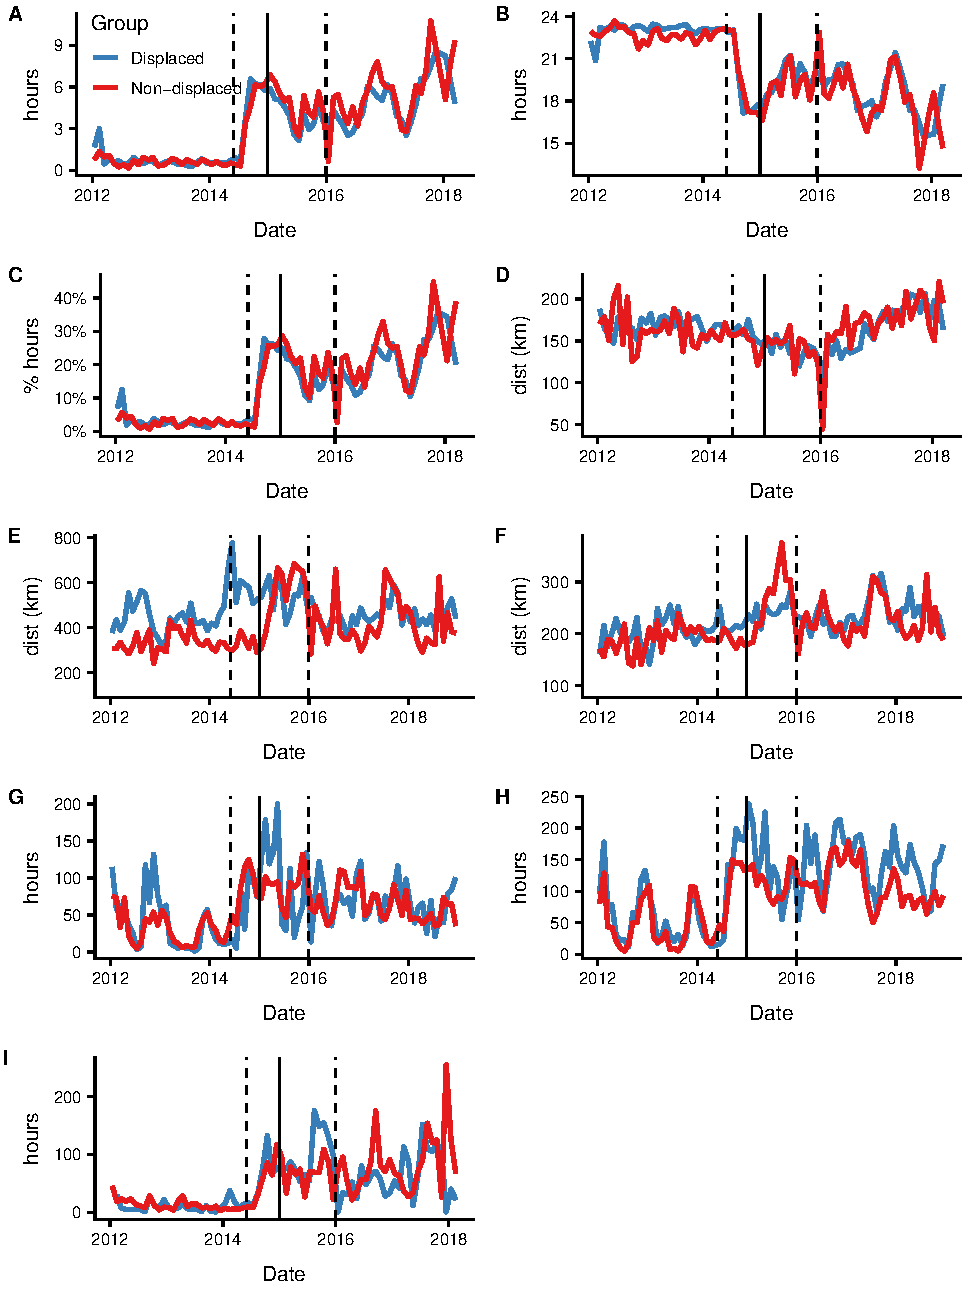
\includegraphics{img/all_panels.pdf}
	\caption{\label{fig:all_panels}Time series showing monthly averages for our nine variables of interest: A) Fishing hours, B) Non-fishing hours at-sea, C) Proportion of fishing hours to total hours at-sea, D) Distance traveled, E) Mean distance from port for fishing events, F) Mean distance from shore for fishing events, G) Monthly hours spent in Kiribati waters, H) Monthly hours spent in PNA waters, I) Monthly hours spent on the high seas. Dashed vertical lines indicate the addition of new AIS satellites. Solid vertical line indicates the closure of PIPA.}
\end{figure}

\begin{figure}
	\centering
	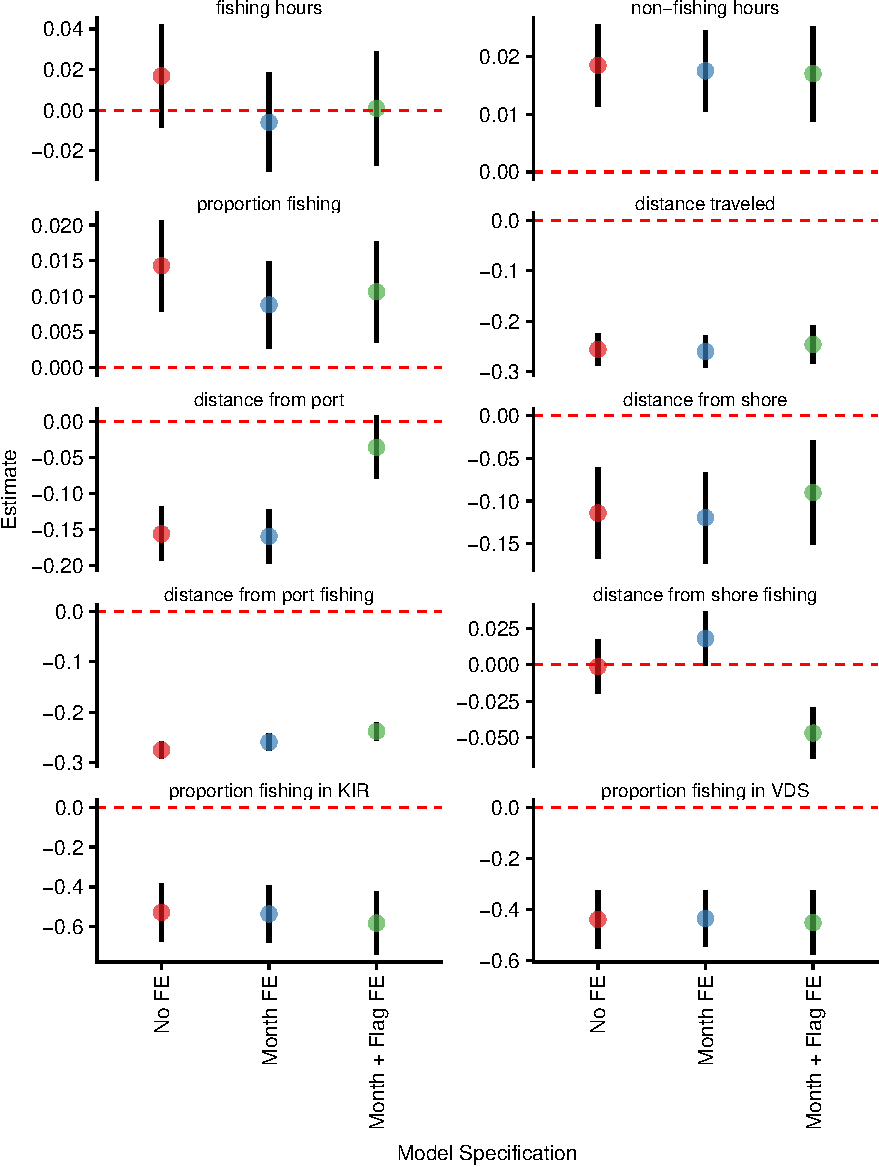
\includegraphics{img/other_specifications.pdf}
	\caption{\label{fig:other_specifications}Alternative difference-in-differences estimates for our variables of interest using different model specifications. Table \ref{tab:main_DID} reports estimates for models with month and flag fixed effects, and NINO4 index (\emph{i.e.} green dots).}
\end{figure}

\begin{landscape}
\begin{table}[H] \centering 
  \caption{\label{tab:DID_without_CHN}Difference-in-differences estimates for our 9 variables of interest after removing Chinese vessels. 1) Daily fishing hours, 2) Daily non-fishing at-sea hours, 3) Daily proportion of fishing hours to total at-sea hours, 4) Daily distance traveled, 5) Daily mean distance from port for fishing events, 6) Daily mean distance from shore for fishing events, 7) Monthly fishing hours spent in Kiribati waters, 8) Monthly fishing hours spent in PNA waters, and 9) Monthly fishing hours in the high seas. Numbers in parentheses are heteroskedastic-robust standard errors.} 
  \label{} 
\footnotesize 
\begin{tabular}{@{\extracolsep{1pt}}lccccccccc} 
\\[-1.8ex]\hline 
\hline \\[-1.8ex] 
\\[-1.8ex] & (1) & (2) & (3) & (4) & (5) & (6) & (7) & (8) & (9)\\ 
\hline \\[-1.8ex] 
 Constant & 0.058$^{***}$ & 3.863$^{***}$ & $-$0.003 & 4.829$^{***}$ & 13.817$^{***}$ & 13.161$^{***}$ & 4.007$^{***}$ & 4.515$^{***}$ & 2.909$^{***}$ \\ 
  & (0.019) & (0.008) & (0.003) & (0.044) & (0.044) & (0.058) & (0.347) & (0.304) & (0.274) \\ 
  & & & & & & & & & \\ 
 Post & 0.824$^{***}$ & $-$0.254$^{***}$ & 0.136$^{***}$ & 0.145$^{***}$ & 0.306$^{***}$ & 0.322$^{***}$ & 0.920$^{***}$ & 1.157$^{***}$ & 0.691$^{**}$ \\ 
  & (0.019) & (0.010) & (0.003) & (0.034) & (0.016) & (0.016) & (0.156) & (0.121) & (0.291) \\ 
  & & & & & & & & & \\ 
 Displaced & 0.108$^{***}$ & 0.009 & 0.012$^{***}$ & 0.270$^{***}$ & 0.271$^{***}$ & 0.158$^{***}$ & 0.491$^{***}$ & 0.150 & $-$0.274 \\ 
  & (0.013) & (0.007) & (0.002) & (0.031) & (0.017) & (0.017) & (0.162) & (0.131) & (0.235) \\ 
  & & & & & & & & & \\ 
 NINO4 & $-$0.012 & $-$0.007 & $-$0.001 & $-$0.380$^{***}$ & 0.164$^{***}$ & 0.061$^{***}$ & 0.365$^{***}$ & 0.122$^{**}$ & 0.464$^{***}$ \\ 
  & (0.011) & (0.005) & (0.002) & (0.018) & (0.009) & (0.008) & (0.074) & (0.060) & (0.126) \\ 
  & & & & & & & & & \\ 
 Post $\times$ Displaced & $-$0.212$^{***}$ & 0.040$^{***}$ & $-$0.031$^{***}$ & $-$0.282$^{***}$ & $-$0.338$^{***}$ & $-$0.205$^{***}$ & $-$0.558$^{***}$ & $-$0.412$^{***}$ & 0.374 \\ 
  & (0.021) & (0.010) & (0.004) & (0.038) & (0.019) & (0.018) & (0.174) & (0.137) & (0.289) \\ 
  & & & & & & & & & \\ 
\hline \\[-1.8ex] 
Month FE & Yes & Yes & Yes & Yes & Yes & Yes & Yes & Yes & Yes \\ 
Flag FE & Yes & Yes & Yes & Yes & Yes & Yes & Yes & Yes & Yes \\ 
Observations & 75,327 & 75,327 & 75,326 & 75,390 & 28,449 & 28,449 & 1,570 & 2,279 & 633 \\ 
R$^{2}$ & 0.102 & 0.073 & 0.108 & 0.017 & 0.075 & 0.091 & 0.128 & 0.209 & 0.266 \\ 
\hline 
\hline \\[-1.8ex] 
\textit{Note:}  & \multicolumn{9}{r}{$^{*}$p$<$0.1; $^{**}$p$<$0.05; $^{***}$p$<$0.01} \\ 
\end{tabular} 
\end{table} 
\end{landscape}

\begin{landscape}
\begin{table}[H] \centering 
  \caption{\label{tab:DID_without_PNA}Difference-in-differences estimates for our 9 variables of interest after removing PNA vessels: 1) Daily fishing hours, 2) Daily non-fishing at-sea hours, 3) Daily proportion of fishing hours to total at-sea hours, 4) Daily distance traveled, 5) Daily mean distance from port for fishing events, 6) Daily mean distance from shore for fishing events, 7) Monthly fishing hours spent in Kiribati waters, 8) Monthly fishing hours spent in PNA waters, and 9) Monthly fishing hours in the high seas. Numbers in parentheses are heteroskedastic-robust standard errors.} 
  \label{} 
\footnotesize 
\begin{tabular}{@{\extracolsep{1pt}}lccccccccc} 
\\[-1.8ex]\hline 
\hline \\[-1.8ex] 
\\[-1.8ex] & (1) & (2) & (3) & (4) & (5) & (6) & (7) & (8) & (9)\\ 
\hline \\[-1.8ex] 
 Constant & 0.512$^{***}$ & 3.559$^{***}$ & 0.083$^{***}$ & 4.499$^{***}$ & 13.165$^{***}$ & 12.667$^{***}$ & 3.271$^{***}$ & 4.066$^{***}$ & 2.876$^{***}$ \\ 
  & (0.024) & (0.013) & (0.004) & (0.047) & (0.028) & (0.025) & (0.263) & (0.201) & (0.434) \\ 
  & & & & & & & & & \\ 
 Post & 0.781$^{***}$ & $-$0.159$^{***}$ & 0.122$^{***}$ & 0.047 & 0.114$^{***}$ & 0.070$^{***}$ & 1.168$^{***}$ & 1.481$^{***}$ & 0.295 \\ 
  & (0.022) & (0.012) & (0.004) & (0.043) & (0.023) & (0.022) & (0.226) & (0.180) & (0.333) \\ 
  & & & & & & & & & \\ 
 Displaced & 0.202$^{***}$ & 0.040$^{***}$ & 0.019$^{***}$ & 0.437$^{***}$ & 0.165$^{***}$ & $-$0.015 & 0.817$^{***}$ & 0.533$^{***}$ & $-$0.408$^{*}$ \\ 
  & (0.015) & (0.009) & (0.003) & (0.037) & (0.024) & (0.022) & (0.229) & (0.182) & (0.235) \\ 
  & & & & & & & & & \\ 
 NINO4 & $-$0.019 & $-$0.0003 & $-$0.002 & $-$0.387$^{***}$ & 0.138$^{***}$ & 0.025$^{***}$ & 0.413$^{***}$ & 0.232$^{***}$ & 0.482$^{***}$ \\ 
  & (0.012) & (0.006) & (0.002) & (0.020) & (0.010) & (0.009) & (0.080) & (0.066) & (0.156) \\ 
  & & & & & & & & & \\ 
 Post $\times$ Displaced & $-$0.219$^{***}$ & $-$0.055$^{***}$ & $-$0.023$^{***}$ & $-$0.246$^{***}$ & $-$0.175$^{***}$ & 0.010 & $-$0.843$^{***}$ & $-$0.821$^{***}$ & 0.729$^{**}$ \\ 
  & (0.024) & (0.012) & (0.004) & (0.046) & (0.026) & (0.024) & (0.243) & (0.195) & (0.341) \\ 
  & & & & & & & & & \\ 
\hline \\[-1.8ex] 
Month FE & Yes & Yes & Yes & Yes & Yes & Yes & Yes & Yes & Yes \\ 
Flag FE & Yes & Yes & Yes & Yes & Yes & Yes & Yes & Yes & Yes \\ 
Observations & 64,560 & 64,560 & 64,559 & 64,625 & 22,654 & 22,654 & 1,366 & 1,928 & 511 \\ 
R$^{2}$ & 0.093 & 0.069 & 0.099 & 0.022 & 0.063 & 0.066 & 0.127 & 0.203 & 0.214 \\ 
\hline 
\hline \\[-1.8ex] 
\textit{Note:}  & \multicolumn{9}{r}{$^{*}$p$<$0.1; $^{**}$p$<$0.05; $^{***}$p$<$0.01} \\ 
\end{tabular} 
\end{table} 
\end{landscape}

\begin{landscape}
\begin{table}[H] \centering 
  \caption{\label{tab:DID_without_USA_TWN}Difference-in-differences estimates for our 9 variables of interest after removing US and Tawianese vessels. 1) Daily fishing hours, 2) Daily non-fishing at-sea hours, 3) Daily proportion of fishing hours to total at-sea hours, 4) Daily distance traveled, 5) Daily mean distance from port for fishing events, 6) Daily mean distance from shore for fishing events, 7) Monthly fishing hours spent in Kiribati waters, 8) Monthly fishing hours spent in PNA waters, and 9) Monthly fishing hours in the high seas. Numbers in parentheses are heteroskedastic-robust standard errors.} 
  \label{} 
\footnotesize 
\begin{tabular}{@{\extracolsep{1pt}}lccccccccc} 
\\[-1.8ex]\hline 
\hline \\[-1.8ex] 
\\[-1.8ex] & (1) & (2) & (3) & (4) & (5) & (6) & (7) & (8) & (9)\\ 
\hline \\[-1.8ex] 
 Constant & 0.536$^{***}$ & 3.600$^{***}$ & 0.082$^{***}$ & 4.506$^{***}$ & 13.002$^{***}$ & 12.438$^{***}$ & 3.850$^{***}$ & 4.719$^{***}$ & 2.420$^{***}$ \\ 
  & (0.023) & (0.012) & (0.004) & (0.043) & (0.022) & (0.020) & (0.209) & (0.158) & (0.419) \\ 
  & & & & & & & & & \\ 
 Post & 0.796$^{***}$ & $-$0.217$^{***}$ & 0.130$^{***}$ & 0.021 & 0.290$^{***}$ & 0.291$^{***}$ & 0.870$^{***}$ & 0.894$^{***}$ & 0.732$^{**}$ \\ 
  & (0.019) & (0.010) & (0.003) & (0.035) & (0.016) & (0.016) & (0.156) & (0.121) & (0.291) \\ 
  & & & & & & & & & \\ 
 Displaced & 0.142$^{***}$ & 0.016$^{**}$ & 0.015$^{***}$ & 0.341$^{***}$ & 0.227$^{***}$ & 0.127$^{***}$ & 0.490$^{***}$ & $-$0.017 & $-$0.296 \\ 
  & (0.013) & (0.007) & (0.002) & (0.031) & (0.018) & (0.017) & (0.163) & (0.126) & (0.239) \\ 
  & & & & & & & & & \\ 
 NINO4 & $-$0.001 & $-$0.001 & 0.001 & $-$0.383$^{***}$ & 0.189$^{***}$ & 0.082$^{***}$ & 0.325$^{***}$ & 0.171$^{***}$ & 0.441$^{***}$ \\ 
  & (0.011) & (0.006) & (0.002) & (0.019) & (0.009) & (0.008) & (0.075) & (0.063) & (0.122) \\ 
  & & & & & & & & & \\ 
 Post $\times$ Displaced & $-$0.212$^{***}$ & $-$0.002 & $-$0.029$^{***}$ & $-$0.158$^{***}$ & $-$0.328$^{***}$ & $-$0.184$^{***}$ & $-$0.533$^{***}$ & $-$0.225 & 0.339 \\ 
  & (0.021) & (0.010) & (0.004) & (0.039) & (0.019) & (0.018) & (0.175) & (0.138) & (0.291) \\ 
  & & & & & & & & & \\ 
\hline \\[-1.8ex] 
Month FE & Yes & Yes & Yes & Yes & Yes & Yes & Yes & Yes & Yes \\ 
Flag FE & Yes & Yes & Yes & Yes & Yes & Yes & Yes & Yes & Yes \\ 
Observations & 73,717 & 73,717 & 73,716 & 73,778 & 26,920 & 26,920 & 1,546 & 2,236 & 660 \\ 
R$^{2}$ & 0.095 & 0.072 & 0.102 & 0.021 & 0.077 & 0.094 & 0.111 & 0.169 & 0.256 \\ 
\hline 
\hline \\[-1.8ex] 
\textit{Note:}  & \multicolumn{9}{r}{$^{*}$p$<$0.1; $^{**}$p$<$0.05; $^{***}$p$<$0.01} \\ 
\end{tabular} 
\end{table} 
\end{landscape}

\begin{landscape}
\begin{table}[H] \centering 
  \caption{\label{tab:sp_corr}Coefficient estimates for a fourth-degree polynomial fit to the measures of crowding for all PNA waters. The first five columns represent different specifications for number of cells with presence of both fleets. Columns 6 - 10 show coefficients for the spatial correlation for presence / absence of displaced and non-displaced vessels. The explanatory variable is the number of months before or after implementation of PIPA. Numbers in parentheses are heteroskedastic-robust standard errors. The last column of each group presents fits with only NINO4 anomaly index as an explanatory variable.} 
  \label{} 
\footnotesize 
\begin{tabular}{@{\extracolsep{0.1pt}}lcccccccccc} 
\\[-1.8ex]\hline 
\hline \\[-1.8ex] 
\\[-1.8ex] & \multicolumn{5}{c}{Number of cells} & \multicolumn{5}{c}{Pearson's correlation coefficient} \\ 
\\[-1.8ex] & (1) & (2) & (3) & (4) & (5) & (6) & (7) & (8) & (9) & (10)\\ 
\hline \\[-1.8ex] 
 Constant & 78.04$^{***}$ & 84.64$^{***}$ & 60.96$^{***}$ & 66.73$^{***}$ & 80.62$^{***}$ & 0.41$^{***}$ & 0.42$^{***}$ & 0.37$^{***}$ & 0.38$^{***}$ & 0.38$^{***}$ \\ 
  & (5.44) & (8.99) & (15.60) & (15.99) & (7.96) & (0.01) & (0.03) & (0.06) & (0.07) & (0.02) \\ 
  & & & & & & & & & & \\ 
 M & 3.94$^{***}$ & 4.07$^{***}$ & 3.07$^{***}$ & 3.14$^{***}$ &  & 0.01$^{***}$ & 0.01$^{***}$ & 0.01$^{**}$ & 0.01$^{**}$ &  \\ 
  & (0.30) & (0.35) & (0.97) & (1.04) &  & (0.001) & (0.001) & (0.003) & (0.004) &  \\ 
  & & & & & & & & & & \\ 
 M $^2$ & $-$0.005 & $-$0.02 & 0.01 & $-$0.01 &  & $-$0.0001$^{***}$ & $-$0.0001 & $-$0.0001 & $-$0.0001 &  \\ 
  & (0.02) & (0.03) & (0.03) & (0.03) &  & (0.0000) & (0.0001) & (0.0001) & (0.0001) &  \\ 
  & & & & & & & & & & \\ 
 M $^3$ & $-$0.002$^{***}$ & $-$0.002$^{***}$ & $-$0.002$^{***}$ & $-$0.002$^{***}$ &  & $-$0.0000$^{***}$ & $-$0.0000$^{***}$ & $-$0.0000$^{***}$ & $-$0.0000$^{***}$ &  \\ 
  & (0.0003) & (0.0003) & (0.001) & (0.001) &  & (0.0000) & (0.0000) & (0.0000) & (0.0000) &  \\ 
  & & & & & & & & & & \\ 
 M $^4$ & 0.0000 & 0.0000 & 0.0000 & 0.0000 &  & 0.0000$^{***}$ & 0.0000$^{**}$ & 0.0000 & 0.0000 &  \\ 
  & (0.0000) & (0.0000) & (0.0000) & (0.0000) &  & (0.0000) & (0.0000) & (0.0000) & (0.0000) &  \\ 
  & & & & & & & & & & \\ 
 NINO4 &  & $-$8.09 &  & $-$10.39 & 19.76$^{**}$ &  & $-$0.01 &  & $-$0.01 & 0.07$^{***}$ \\ 
  &  & (8.29) &  & (9.48) & (9.41) &  & (0.03) &  & (0.03) & (0.02) \\ 
  & & & & & & & & & & \\ 
 $\sigma_1$ &  &  & 21.32 & 25.10 &  &  &  & 0.06 & 0.06 &  \\ 
  &  &  & (19.49) & (22.49) &  &  &  & (0.08) & (0.08) &  \\ 
  & & & & & & & & & & \\ 
 $\sigma_2$ &  &  & 5.30 & 3.19 &  &  &  & $-$0.01 & $-$0.02 &  \\ 
  &  &  & (18.87) & (18.67) &  &  &  & (0.04) & (0.03) &  \\ 
  & & & & & & & & & & \\ 
\hline \\[-1.8ex] 
NINO4 & No & Yes & No & Yes & Yes & No & Yes & No & Yes & Yes \\ 
Satellites & No & No & Yes & Yes & No &  &  &  &  &  \\ 
AIC & 796.937 & 797.991 & 799.477 & 799.97 & 919.583 & -187.208 & -185.269 & -184.916 & -183.233 & -97.386 \\ 
Observations & 84 & 84 & 84 & 84 & 84 & 84 & 84 & 84 & 84 & 84 \\ 
R$^{2}$ & 0.79 & 0.79 & 0.79 & 0.80 & 0.03 & 0.70 & 0.70 & 0.71 & 0.71 & 0.07 \\ 
\hline 
\hline \\[-1.8ex] 
\textit{Note:}  & \multicolumn{10}{r}{$^{*}$p$<$0.1; $^{**}$p$<$0.05; $^{***}$p$<$0.01} \\ 
\end{tabular} 
\end{table} 
\end{landscape}

\begin{figure}[htbp]
\centering
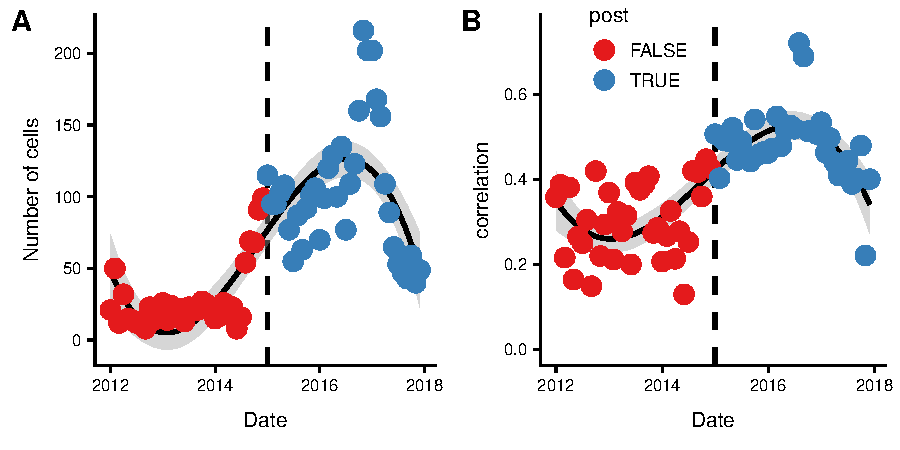
\includegraphics{img/sp_corr.pdf}
\caption{\label{fig:sp_corr}Number of cells that had displaced and non-displaced vessels (A) and spatial correlation in the presence-absence of each group per cell (B). The solid lines represent the 4\textsuperscript{th} degree polynomial fit reported in \ref{tab:sp_corr}. Note that the late 2016 and early 2017 showed negative or neutral NINO4 anomalies similar to those in the pre-PIPA period, but crowding effect does not decline to pre-implementation level and seems to stabilize.}
\end{figure}

\begin{landscape}
\begin{table}[H] \centering 
  \caption{\label{tab:KIR_sp_corr}Coefficient estimates for a fourth-degree polynomial fit to the measures of crowding for Kiribati EEZ only. The first five columns represent different specifications for number of cells with presence of both fleets. Columns 6 - 10 show coefficients for the spatial correlation for presence / absence of displaced and non-displaced vessels. The explanatory variable is the number of months before or after implementation of PIPA. Numbers in parentheses are heteroskedastic-robust standard errors. The last column of each group presents fits with only NINO4 anomaly index as an explanatory variable.} 
  \label{} 
\footnotesize 
\begin{tabular}{@{\extracolsep{0.1pt}}lcccccccccc} 
\\[-1.8ex]\hline 
\hline \\[-1.8ex] 
\\[-1.8ex] & \multicolumn{5}{c}{Number of cells} & \multicolumn{5}{c}{Pearson's correlation coefficient} \\ 
\\[-1.8ex] & (1) & (2) & (3) & (4) & (5) & (6) & (7) & (8) & (9) & (10)\\ 
\hline \\[-1.8ex] 
 Constant & 30.24$^{***}$ & 32.77$^{***}$ & 23.30$^{***}$ & 26.14$^{***}$ & 16.23$^{***}$ & 0.43$^{***}$ & 0.43$^{***}$ & 0.33$^{***}$ & 0.34$^{***}$ & 0.38$^{***}$ \\ 
  & (2.43) & (4.16) & (4.59) & (5.49) & (2.37) & (0.03) & (0.05) & (0.07) & (0.08) & (0.03) \\ 
  & & & & & & & & & & \\ 
 M & 1.29$^{***}$ & 1.34$^{***}$ & 1.00$^{***}$ & 1.06$^{***}$ &  & 0.01$^{***}$ & 0.01$^{***}$ & 0.01$^{*}$ & 0.01 &  \\ 
  & (0.14) & (0.17) & (0.27) & (0.30) &  & (0.002) & (0.002) & (0.01) & (0.01) &  \\ 
  & & & & & & & & & & \\ 
 M $^2$ & $-$0.03$^{***}$ & $-$0.04$^{***}$ & $-$0.02$^{**}$ & $-$0.03$^{***}$ &  & 0.0000 & 0.0000 & 0.0001 & 0.0001 &  \\ 
  & (0.01) & (0.01) & (0.01) & (0.01) &  & (0.0002) & (0.0002) & (0.0002) & (0.0002) &  \\ 
  & & & & & & & & & & \\ 
 M $^3$ & $-$0.001$^{***}$ & $-$0.001$^{***}$ & $-$0.001$^{***}$ & $-$0.001$^{***}$ &  & $-$0.0000$^{***}$ & $-$0.0000$^{***}$ & $-$0.0000$^{**}$ & $-$0.0000$^{**}$ &  \\ 
  & (0.0001) & (0.0001) & (0.0002) & (0.0002) &  & (0.0000) & (0.0000) & (0.0000) & (0.0000) &  \\ 
  & & & & & & & & & & \\ 
 M $^4$ & 0.0000$^{***}$ & 0.0000$^{***}$ & 0.0000$^{**}$ & 0.0000$^{***}$ &  & $-$0.0000 & $-$0.0000 & $-$0.0000 & $-$0.0000 &  \\ 
  & (0.0000) & (0.0000) & (0.0000) & (0.0000) &  & (0.0000) & (0.0000) & (0.0000) & (0.0000) &  \\ 
  & & & & & & & & & & \\ 
 NINO4 &  & $-$3.10 &  & $-$4.19 & 9.93$^{***}$ &  & $-$0.001 &  & $-$0.02 & 0.11$^{***}$ \\ 
  &  & (3.97) &  & (4.16) & (3.33) &  & (0.05) &  & (0.06) & (0.03) \\ 
  & & & & & & & & & & \\ 
 $\sigma_1$ &  &  & 9.40 & 10.33 &  &  &  & 0.12 & 0.13 &  \\ 
  &  &  & (5.92) & (6.35) &  &  &  & (0.09) & (0.09) &  \\ 
  & & & & & & & & & & \\ 
 $\sigma_2$ &  &  & $-$2.46 & $-$3.84 &  &  &  & 0.02 & 0.01 &  \\ 
  &  &  & (5.70) & (5.77) &  &  &  & (0.10) & (0.11) &  \\ 
  & & & & & & & & & & \\ 
\hline \\[-1.8ex] 
NINO4 & No & Yes & No & Yes & Yes & No & Yes & No & Yes & Yes \\ 
Satellites & No & No & Yes & Yes & No &  &  &  &  &  \\ 
AIC & 654.294 & 655.536 & 655.482 & 656.125 & 724.58 & -65.872 & -63.873 & -63.481 & -61.572 & -35.895 \\ 
Observations & 84 & 84 & 84 & 84 & 84 & 75 & 75 & 75 & 75 & 75 \\ 
R$^{2}$ & 0.63 & 0.63 & 0.64 & 0.65 & 0.08 & 0.44 & 0.44 & 0.45 & 0.45 & 0.09 \\ 
\hline 
\hline \\[-1.8ex] 
\textit{Note:}  & \multicolumn{10}{r}{$^{*}$p$<$0.1; $^{**}$p$<$0.05; $^{***}$p$<$0.01} \\ 
\end{tabular} 
\end{table} 
\end{landscape}

\begin{figure}
\centering
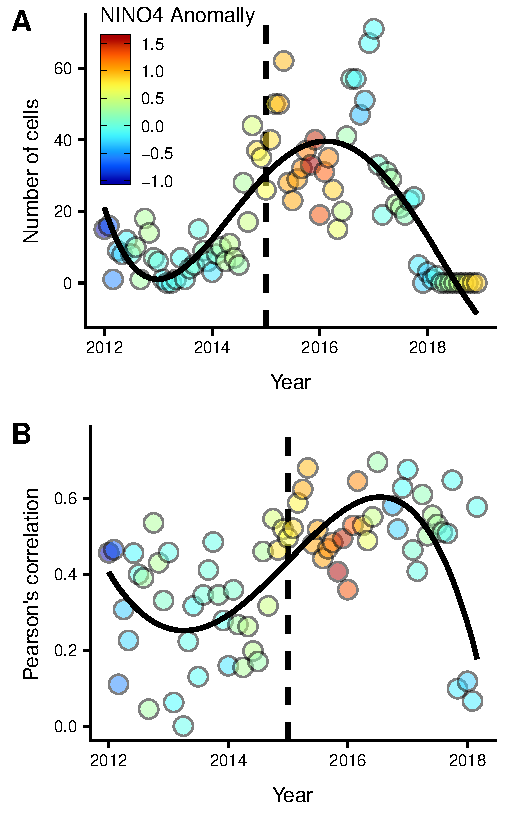
\includegraphics{img/KIR_sp_corr.pdf}
\caption{\label{fig:KIR_sp_corr}Number of cells that had displaced and non-displaced vessels (A) and spatial correlation in the presence-absence of each group per cell (B) for Kiribati's EEZ only. The solid lines represent the 4\textsuperscript{th} degree polynomial fit reported in \ref{tab:sp_corr}. Note that the late 2016 and early 2017 showed negative or neutral NINO4 anomalies, similar to those in the pre-PIPA period.}
\end{figure}



\begin{figure}
\centering
	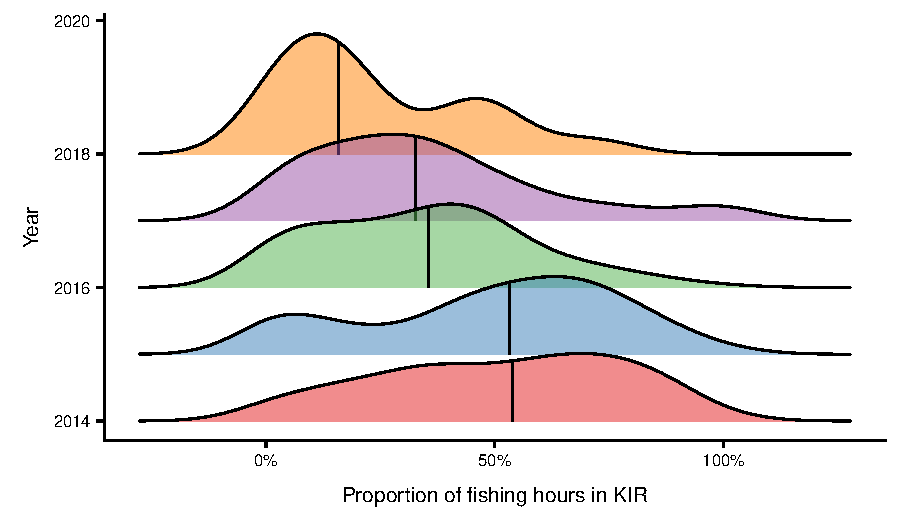
\includegraphics{img/hist_kir_fishing.pdf}
	\caption{\label{fig:hist_kir_fishing}Ridgeplot for the density of the \% of total fishing hours that take place within Kiribati EEZ waters by year for displaced vessels where the unit of observation is an individual vessel.}	
\end{figure}

\begin{figure}
\centering
	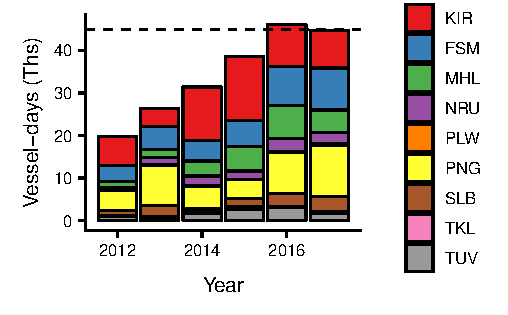
\includegraphics{img/all_PS_VDS_cty_year.pdf}
	\caption{\label{fig:all_PS_VDS_cty_year}Annual vessel-days for all PNA countries, by country.}
\end{figure}

\begin{figure}
\centering
	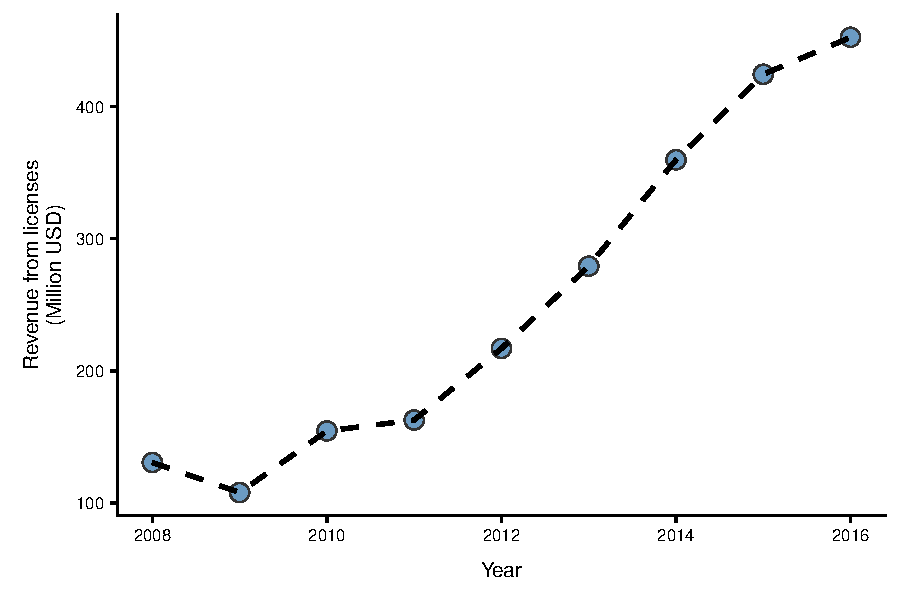
\includegraphics{img/total_PNA_revenues.pdf}
	\caption{\label{fig:total_PNA_revenues}Total revenues for all PNA countries combined.}
\end{figure}

\begin{figure}
\centering
	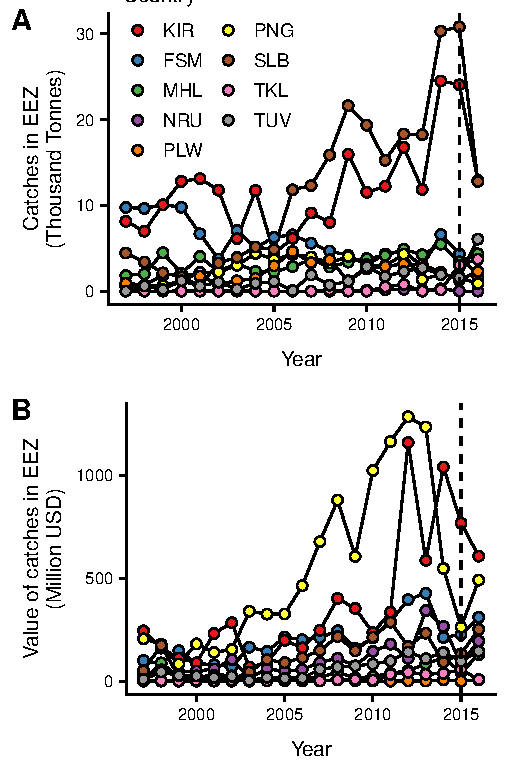
\includegraphics{img/catches.pdf}
	\caption{\label{fig:catches}Financial indicators for PNA countries. A) Total annual purse seine catch by EEZ and, B) Total annual value of purse seine catch by EEZ. Vertical dashed line in both plots denotes implementation of PIPA.}
\end{figure}

\begin{figure}
\centering
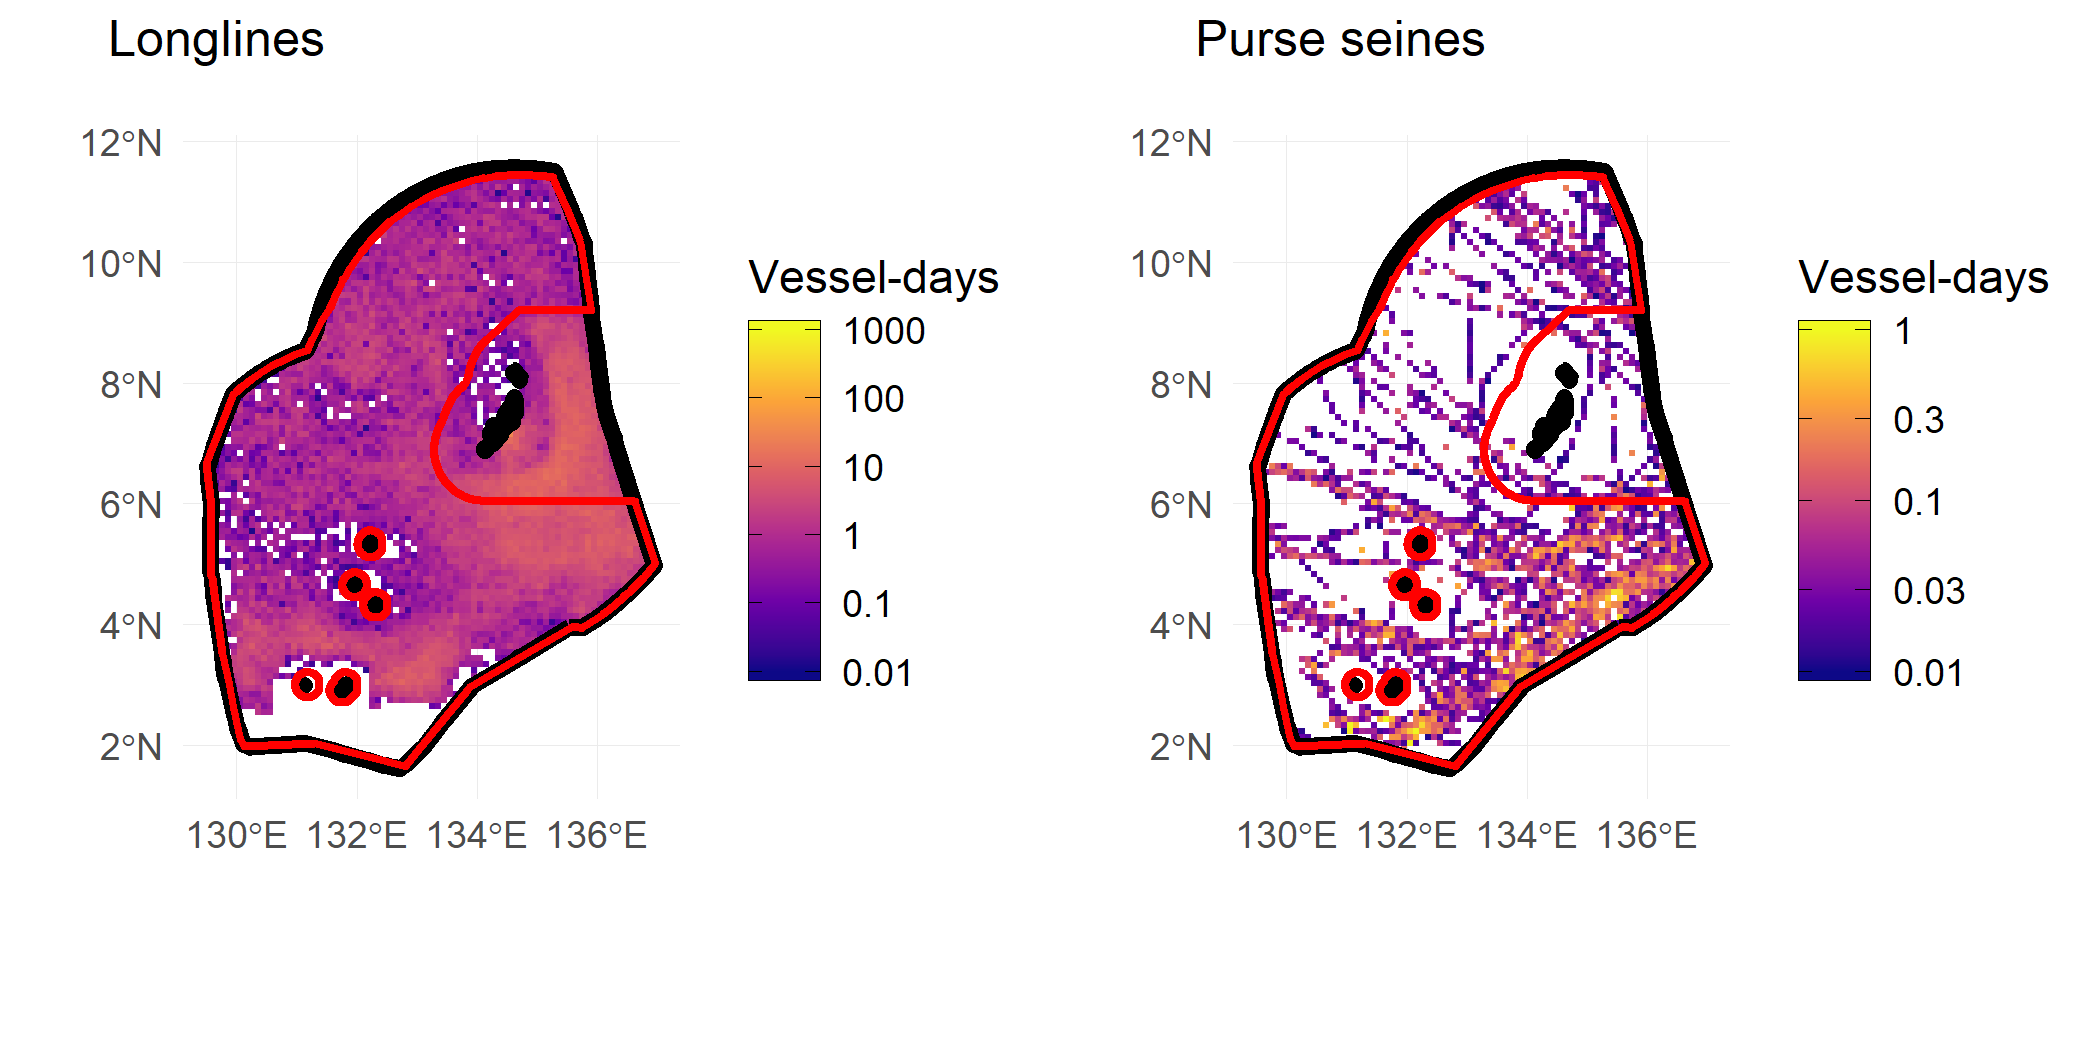
\includegraphics{img/plw_2018.png}
\caption{\label{fig:plw_2018}Longline and purse seine fishing effort in Palau during 2018 at a 0.5 degree resolution. The red polygon shows the proposed Palau National Marine Sanctuary, containing 56\% and 91\% of longline and purse seine fishing effort, respectively. Note that the colorbars are presented in $log_{10}$ transformed scale for better visualization.}
\end{figure}

\begin{figure}
\centering
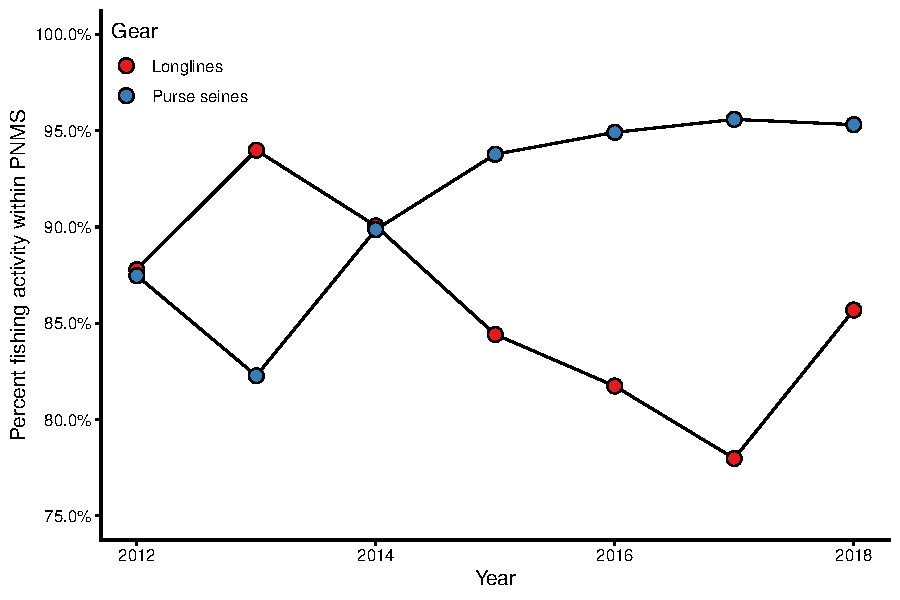
\includegraphics{img/plw_ts_plot.pdf}
\caption{\label{fig:plw_ts_plot}Time series of the annual proportion of longline and purse seine effort within the proposed PNMS boundaries.}
\end{figure}

\clearpage

\bibliography{references}

\bibliographystyle{Science}

\end{document}
